%% Model schematic (PRE Fig. 1). Compile: pdflatex fig_schematic.tex
%% Output is copied to figures/paper/fig_schematic.pdf.
%% Width = PRE column (8.6 cm); fonts 8-9 pt.
\documentclass[tikz,border=2pt]{standalone}
\usepackage{amsmath,amssymb}
\usetikzlibrary{arrows.meta,positioning,calc}
\begin{document}
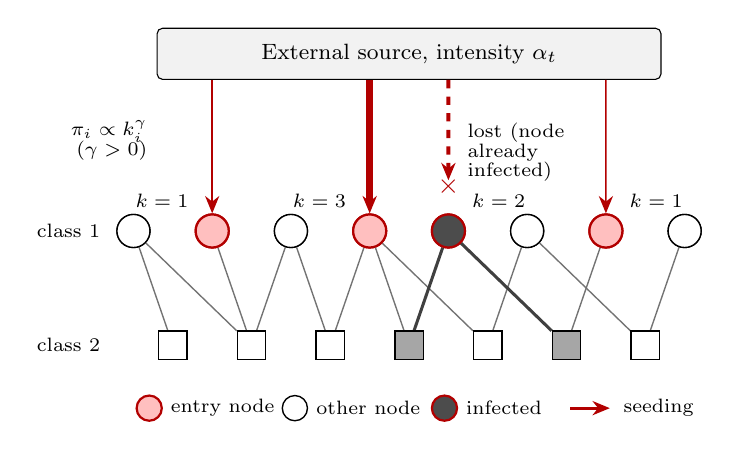
\begin{tikzpicture}[x=1cm,y=1cm,font=\footnotesize,
  c1/.style={circle,draw=black,line width=0.5pt,fill=white,minimum size=4.2mm,inner sep=0},
  c2/.style={rectangle,draw=black,line width=0.5pt,fill=white,minimum size=3.6mm,inner sep=0},
  entry/.style={c1,fill=red!25,draw=red!70!black,line width=0.8pt},
  inf/.style={c1,fill=black!70,draw=red!70!black,line width=0.8pt},
  infsq/.style={c2,fill=black!35},
  edge/.style={line width=0.5pt,black!55},
  infedge/.style={line width=1.1pt,black!75},
  force/.style={-{Stealth[length=2.2mm,width=1.8mm]},red!70!black}]

%% external source
\node[draw=black,rounded corners=2pt,fill=black!5,minimum width=6.4cm,minimum height=6.5mm,
      align=center] (src) at (3.5,2.25) {External source, intensity $\alpha_t$};

%% class 1 (top row) and class 2 (bottom row)
\foreach \i/\x/\s in {1/0.0/c1, 2/1.0/entry, 3/2.0/c1, 4/3.0/entry, 5/4.0/inf, 6/5.0/c1, 7/6.0/entry, 8/7.0/c1}
  \node[\s] (m\i) at (\x,0) {};
\foreach \j/\x in {1/0.5,2/1.5,3/2.5,4/3.5,5/4.5,6/5.5,7/6.5}
  \node[c2] (f\j) at (\x,-1.45) {};

%% partnerships (entry node degrees: m2 -> 1, m4 -> 3, m5 -> 2, m7 -> 1)
\foreach \a/\b in {m1/f1, m2/f2, m3/f2, m3/f3, m4/f3, m4/f4, m4/f5, m6/f5, m7/f6, m8/f7, m6/f7, m1/f2}
  \draw[edge] (\a) -- (\b);
%% m5 was seeded earlier and is infectious; its cluster spreads
\draw[infedge] (m5) -- (f4);
\draw[infedge] (m5) -- (f6);
\node[infsq] at (f4) {};
\node[infsq] at (f6) {};
%% redraw nodes on top of edges
\foreach \i/\s in {1/c1,2/entry,3/c1,4/entry,5/inf,6/c1,7/entry,8/c1}
  \node[\s] at (m\i) {};
\foreach \j in {1,2,3,5,7}
  \node[c2] at (f\j) {};

%% degrees of the entry nodes
\node[above left=0.2mm and 0.2mm of m2,font=\scriptsize] {$k=1$};
\node[above left=0.2mm and 0.2mm of m4,font=\scriptsize] {$k=3$};
\node[above right=0.2mm and 0.2mm of m5,font=\scriptsize] {$k=2$};
\node[above right=0.2mm and 0.2mm of m7,font=\scriptsize] {$k=1$};

%% targeted forcing: arrow width grows with pi_i ~ k^gamma (gamma > 0)
\draw[force,line width=0.6pt] ($(src.south)+(-2.5,0)$) -- (m2.north);
\draw[force,line width=2.4pt] ($(src.south)+(-0.5,0)$) -- (m4.north);
\draw[force,line width=0.6pt] ($(src.south)+(2.5,0)$)  -- (m7.north);
%% seeding aimed at a node that is no longer susceptible: lost
\draw[force,line width=1.4pt,dashed] ($(src.south)+(0.5,0)$) -- ($(m5.north)+(0,0.42)$);
\node[red!70!black,font=\bfseries\normalsize] at ($(m5.north)+(0,0.34)$) {$\times$};
\node[align=left,font=\scriptsize,anchor=west] at (4.12,1.0) {lost (node\\[-1pt]already\\[-1pt]infected)};

\node[font=\scriptsize,anchor=east,align=right] at (0.3,1.15) {$\pi_i\propto k_i^{\gamma}$\\[-1pt]($\gamma>0$)};

%% row labels
\node[anchor=east,font=\scriptsize] at (-0.3,0) {class 1};
\node[anchor=east,font=\scriptsize] at (-0.3,-1.45) {class 2};

%% legend
\begin{scope}[shift={(0.2,-2.25)}]
  \node[entry,minimum size=3.2mm] at (0,0) {};
  \node[anchor=west,font=\scriptsize] at (0.15,0) {entry node};
  \node[c1,minimum size=3.2mm] at (1.85,0) {};
  \node[anchor=west,font=\scriptsize] at (2.0,0) {other node};
  \node[inf,minimum size=3.2mm] at (3.75,0) {};
  \node[anchor=west,font=\scriptsize] at (3.9,0) {infected};
  \draw[force,line width=1pt] (5.35,0) -- (5.85,0);
  \node[anchor=west,font=\scriptsize] at (5.9,0) {seeding};
\end{scope}
\end{tikzpicture}
\end{document}
